\chapter{Additional Material for \cref*{cha:mva}}\label{cha:appendix_mva}

\section{Observables used in the optimization}\label{app:mva:fulllistvars}

\begin{longtable}{ll}
	\caption{List of all observables considered in the optimization of the multivariate analysis.} \\
	\toprule
	  Variable & Description \\
    \midrule
	\endfirsthead
	\caption{List of all observables considered in the optimization of the multivariate analysis (continued).} \\
	\toprule
	  Variable & Description \\
    \midrule
	\endhead
	\bottomrule
	\endfoot
	$\mmc$ & output of the missing mass calculator, see \cref{sub:event_selection:mmc} \\
    $\pt^{ell_1}$           & transverse momentum of the leading lepton \\
    $\eta_{\ell_1}$         & $\eta$ of the leading lepton \\
    $m_\text{T}^{\ell_1}$   & transverse mass of the leading lepton with the transverse energy \\
    $\pt^{ell_2}$           & transverse momentum of the subleading lepton \\
    $\eta_{\ell_2}$         & $\eta$ of the subleading lepton \\
    $m_\text{T}^{\ell_2}$   & transverse mass of the leading lepton with the transverse energy \\
    $n_\text{jets}$         & number of jets above \SI{30}{\GeV}, bins for $n_\text{jets} \geq 3$ are merged\\
    $\pt^{\text{j}_1}$      & transverse momentum of the leading jet \\
    $\eta_{\text{j}_1}$     & $\eta$ of the leading jet \\
    $\pt^{\text{j}_2}$      & transverse momentum of the subleading jet \\
    $\eta_{\text{j}_2}$     & $\eta$ of the subleading jet \\
    $\pt^{\text{j}_3}$      & transverse momentum of the subleading jet \\
    $\eta_{\text{j}_3}$     & $\eta$ of the leading jet \\
    $\mll$                  & invariant mass of the dilepton system \\
    $\etmiss$               & missing transverse energy \\
    $\sum \abs{\pt}$        & scalar sum of $\pt^{\ell_1}$, $\pt^{\ell_2}$, $\pt^{\text{jet}_1}$, $\pt^{\text{jet}_2}$, and $\etmiss$ \\
    $\pt^\text{total}$      & vectorial sum of $\pt^{\ell_1}$, $\pt^{\ell_2}$, $\pt^{\text{jet}_1}$, $\pt^{\text{jet}_2}$, and $\etmiss$\\
    $\etmisshptox$          & $x$ component of the high-$\pt$ object based missing transverse energy \\
    $\etmisshptoy$          & $y$ component of the high-$\pt$ object based missing transverse energy \\
    $\etmisshptophi$        & $\phi$ component of the high-$\pt$ object based missing transverse energy \\
    $x_0^{HPTO}$            & momentum fraction of the leading lepton with respect to the \\
    $x_1^{HPTO}$            & \\
    $\pt^{\tau\tau}$        & \\
    $\pt^{\ell\ell}$        & transverse momentum of the dilepton system \\

\end{longtable}

\section{Correlations of input variables}\label{app:mva:correlation_inputvars}

\begin{figure}[htb]
    \centering
    \begin{subfigure}[t]{0.7\textwidth}
        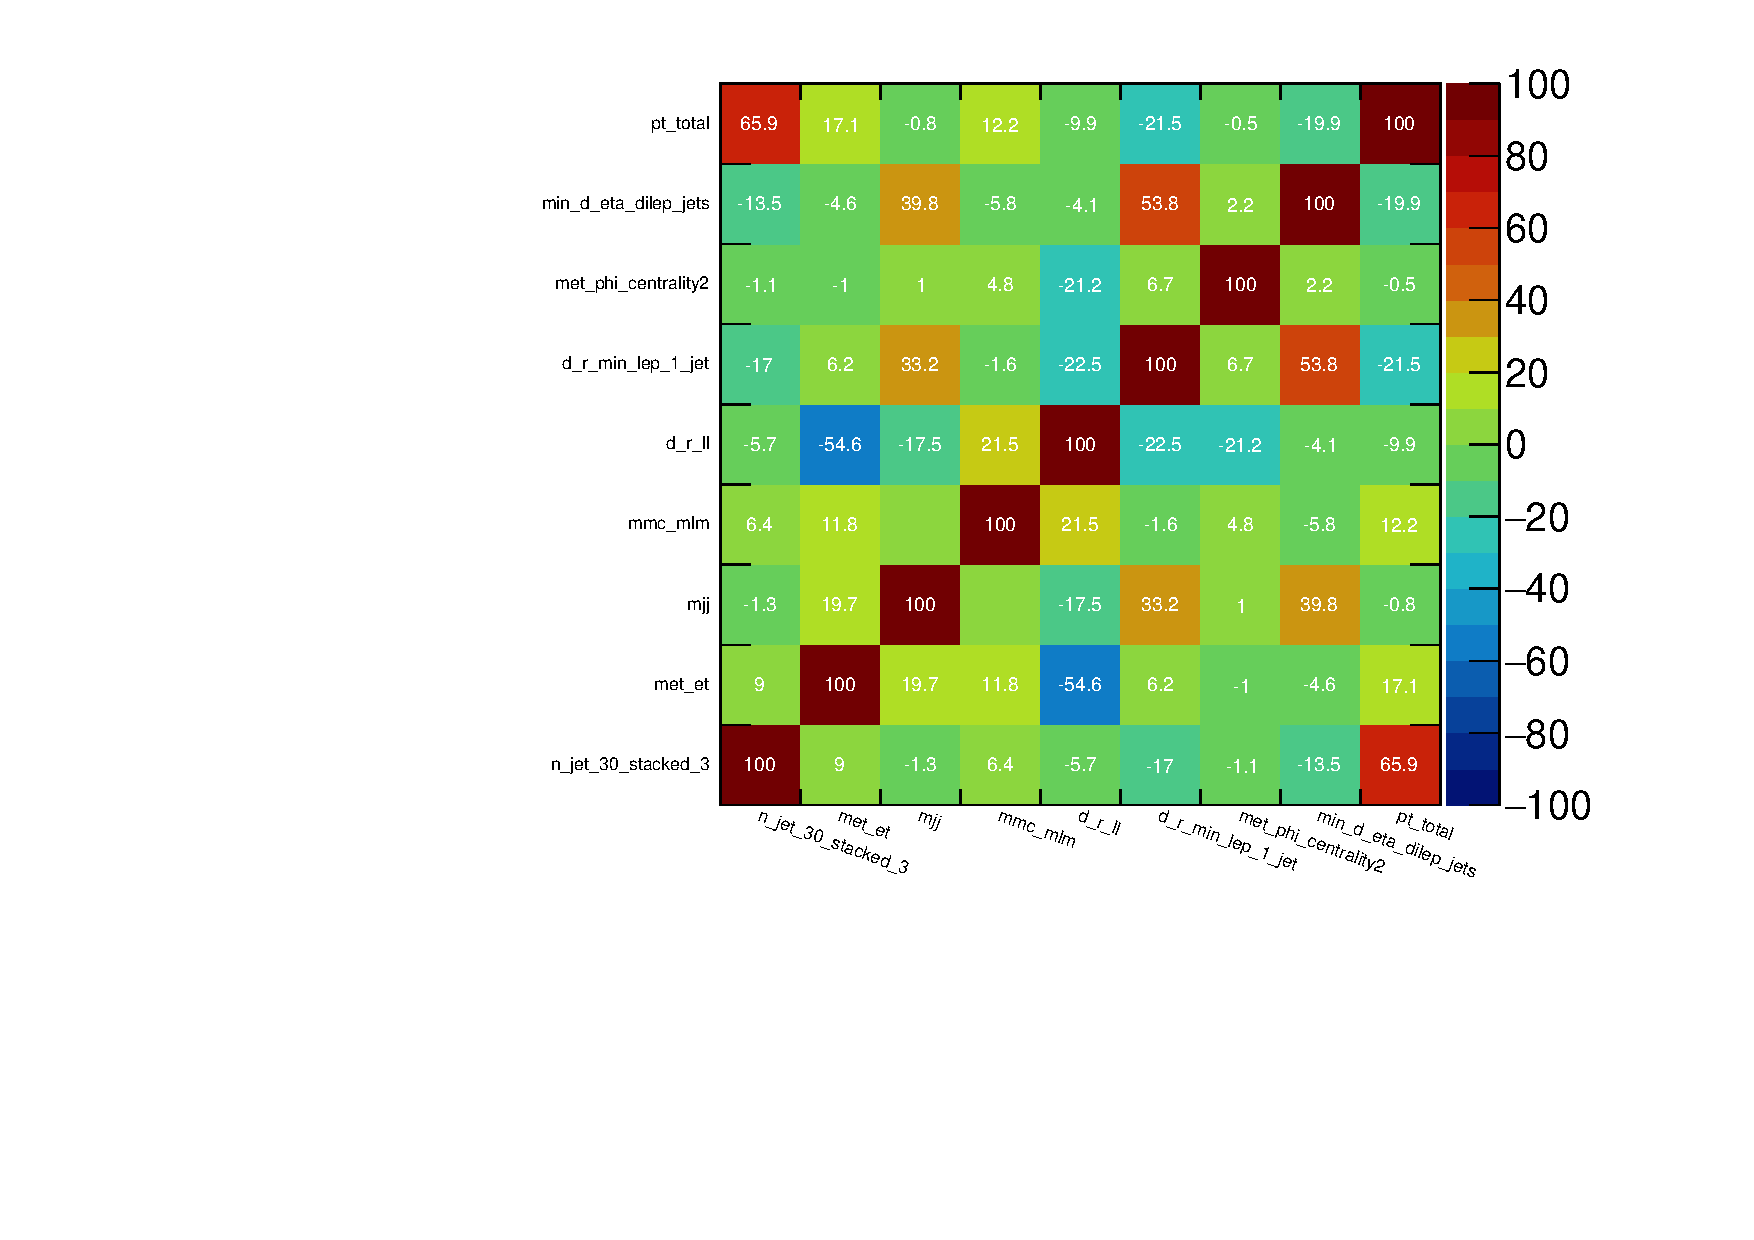
\includegraphics[width=\textwidth]{./plots/mva/variable_reduction/VBF_SF_CorrelationMatrixS.pdf}
        \caption{Signal.}
    \end{subfigure}
    \begin{subfigure}[t]{0.7\textwidth}
        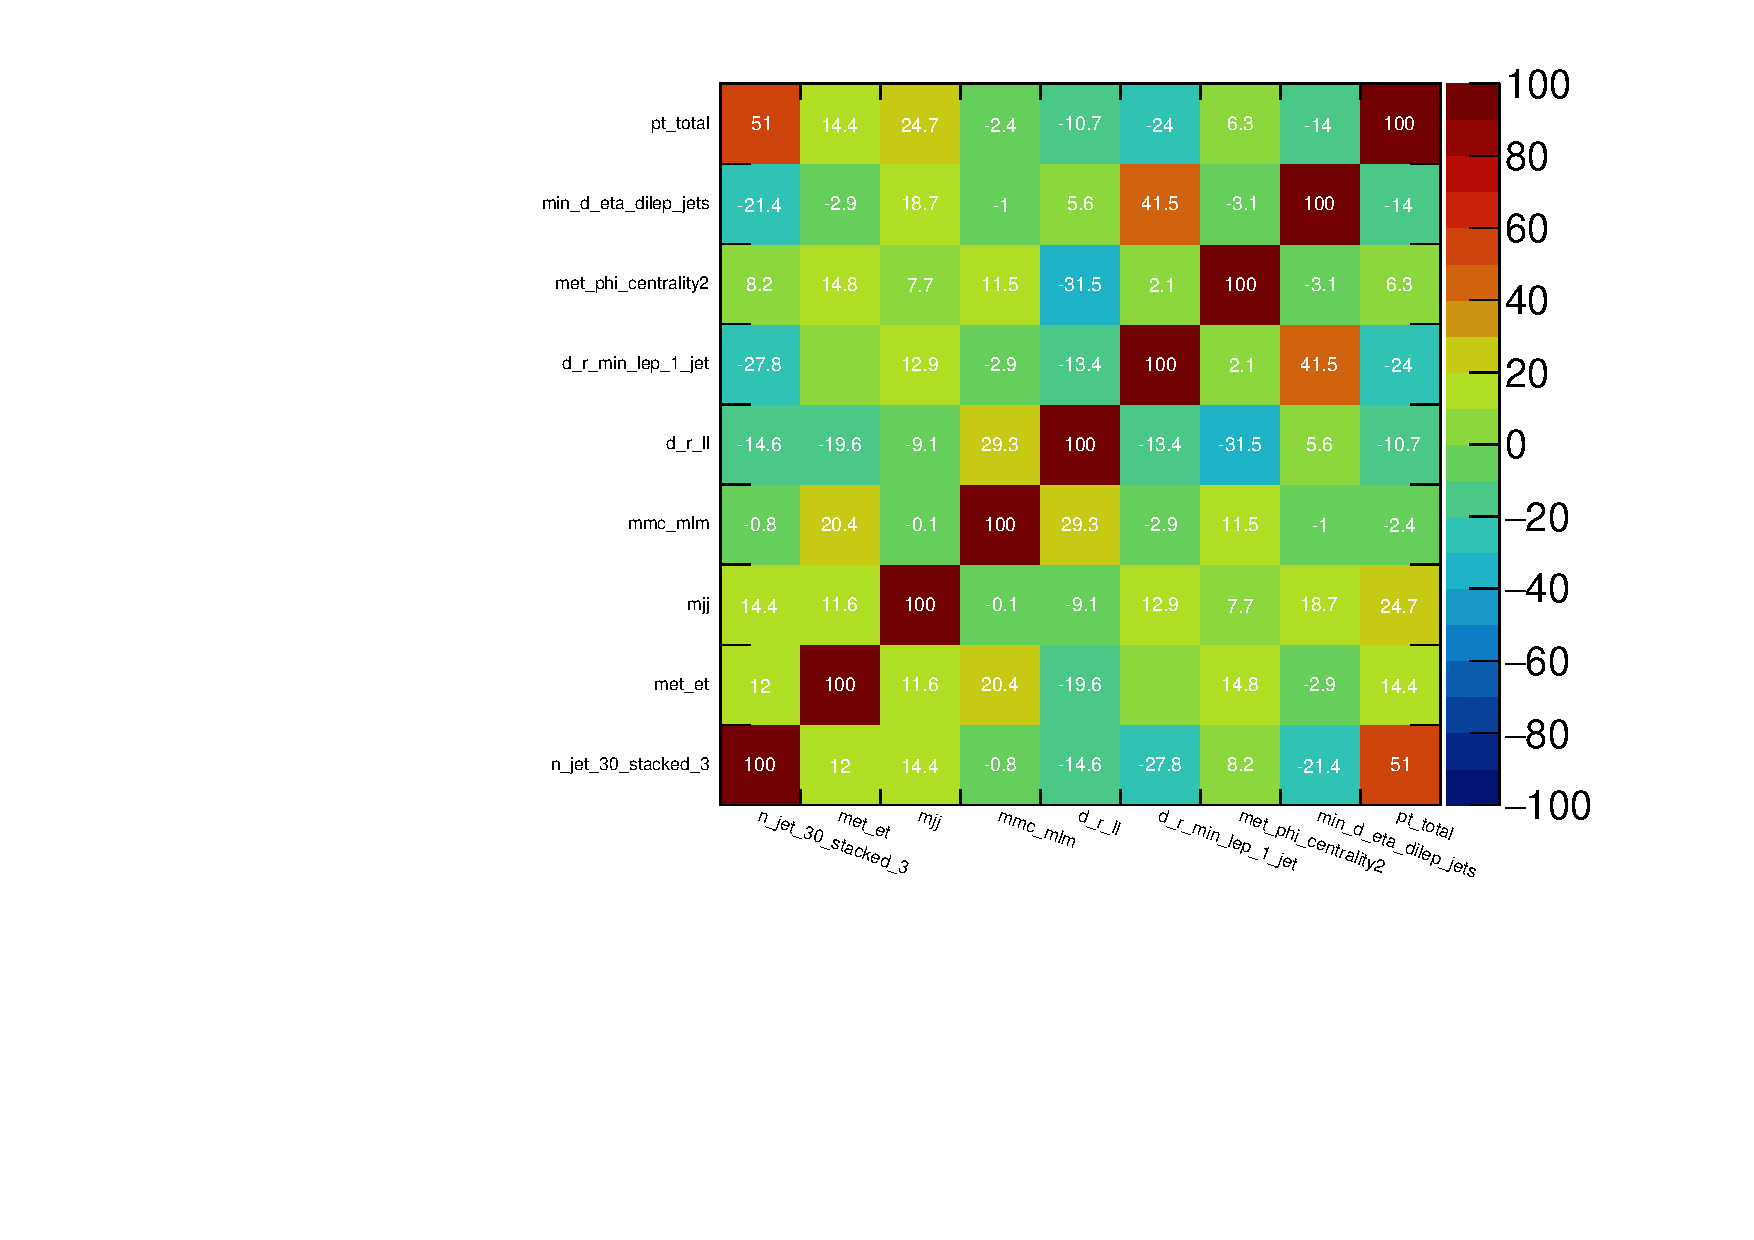
\includegraphics[width=\textwidth]{./plots/mva/variable_reduction/VBF_SF_CorrelationMatrixB.pdf}
        \caption{Background}
    \end{subfigure}
    \caption{Correlations of the input variables for the BDTs in the VBF SF category for signal and background events.}\label{fig:mva:variables:correlationsb:vbfsf}
\end{figure}

\begin{figure}[htb]
    \centering
    \begin{subfigure}[t]{0.7\textwidth}
        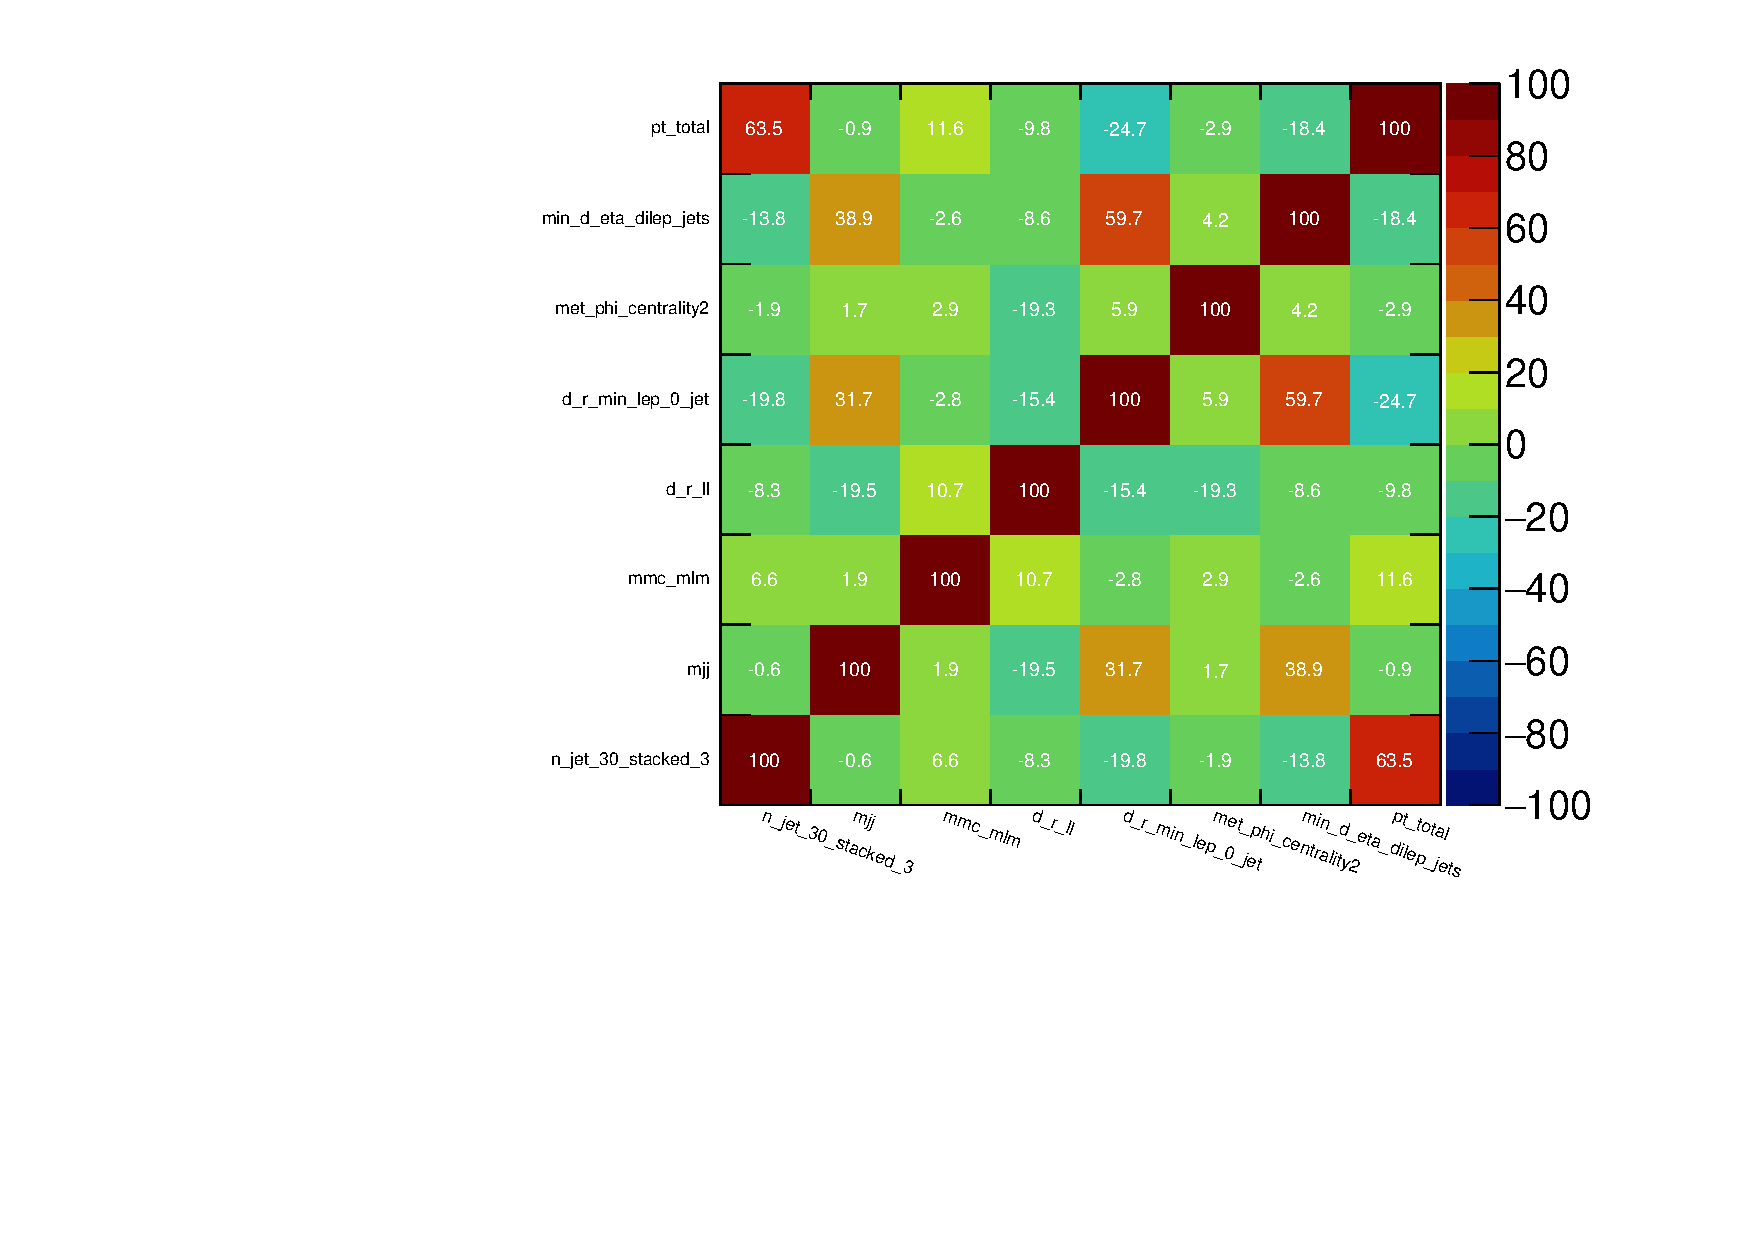
\includegraphics[width=\textwidth]{./plots/mva/variable_reduction/VBF_DF_CorrelationMatrixS.pdf}
        \caption{Signal.}
    \end{subfigure}
    \begin{subfigure}[t]{0.7\textwidth}
        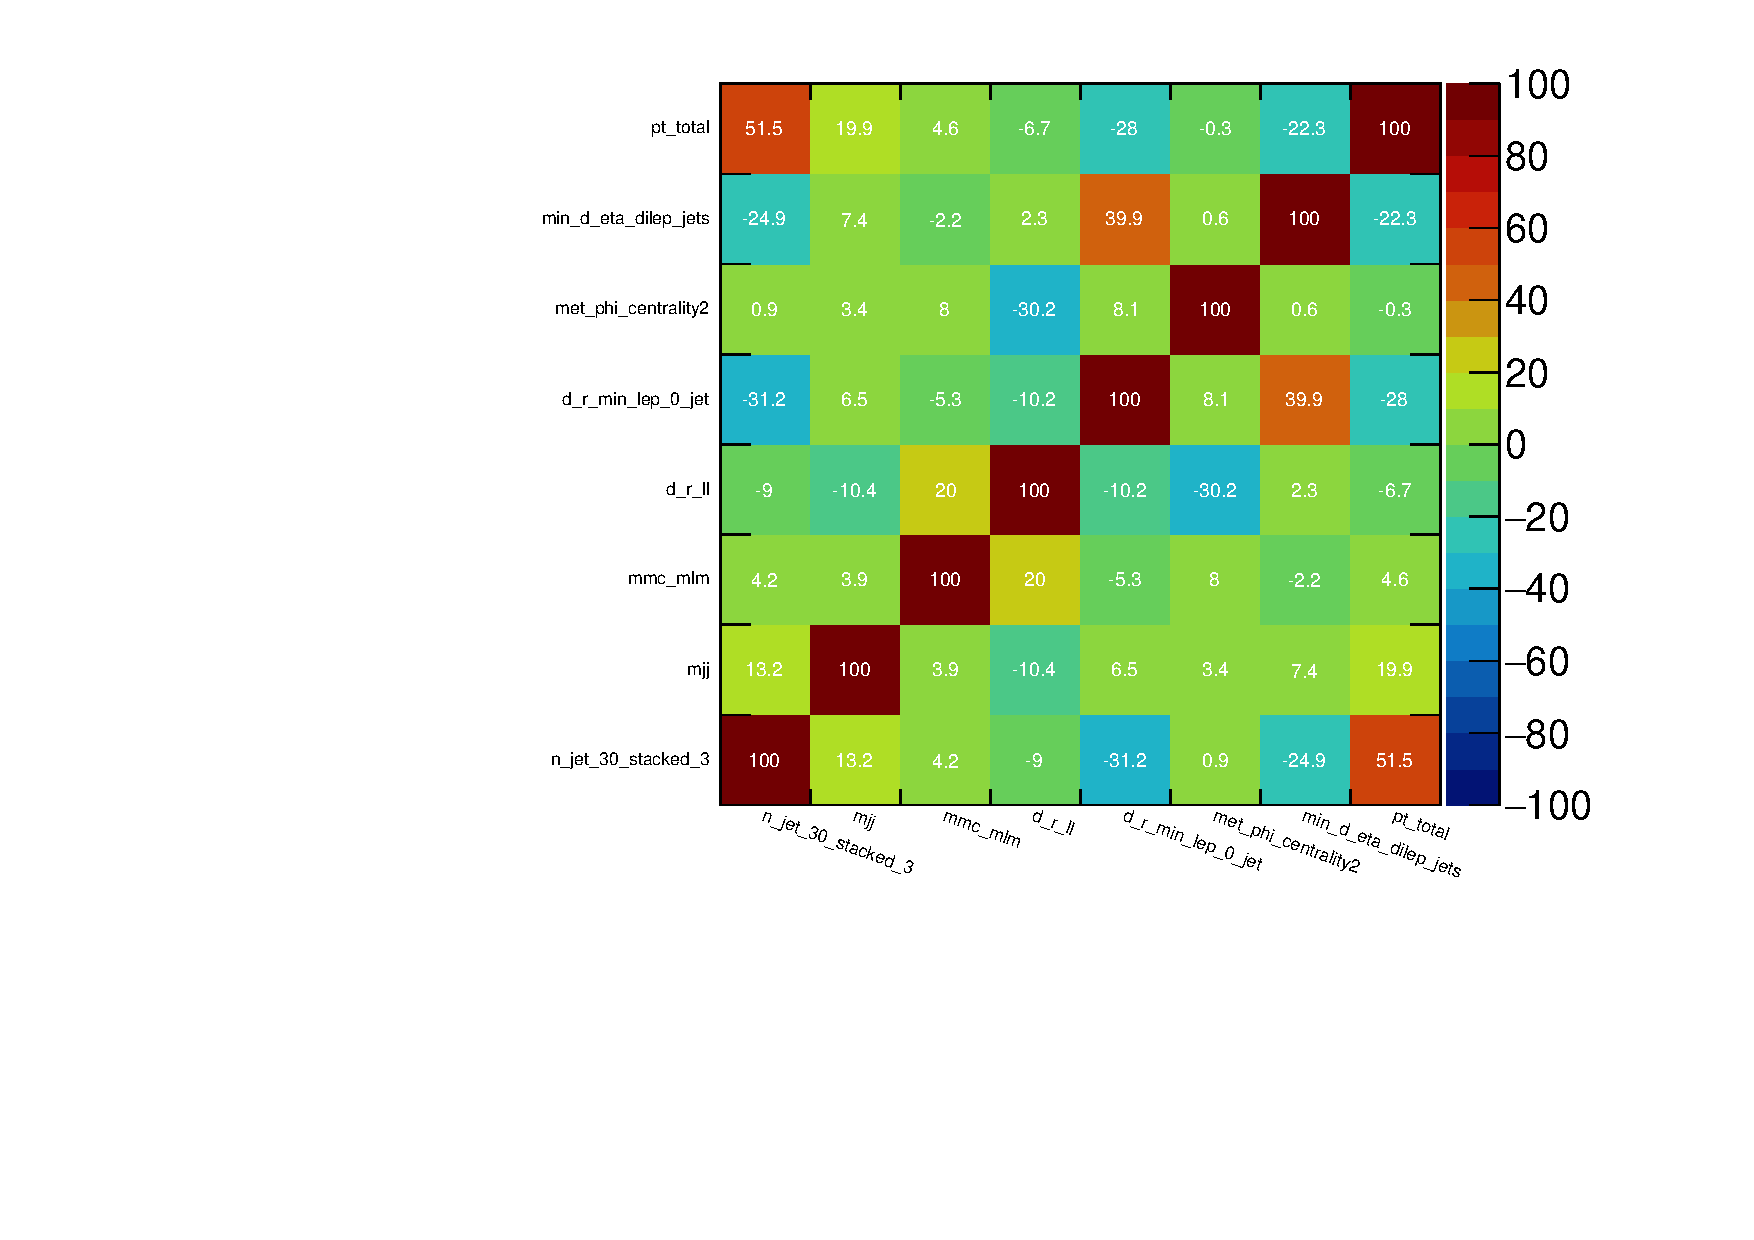
\includegraphics[width=\textwidth]{./plots/mva/variable_reduction/VBF_DF_CorrelationMatrixB.pdf}
        \caption{Background}
    \end{subfigure}
    \caption{Correlations of the input variables for the BDTs in the VBF DF category for signal and background events.}\label{fig:mva:variables:correlationsb:vbfdf}
\end{figure}

\begin{figure}[htb]
    \centering
    \begin{subfigure}[t]{0.7\textwidth}
        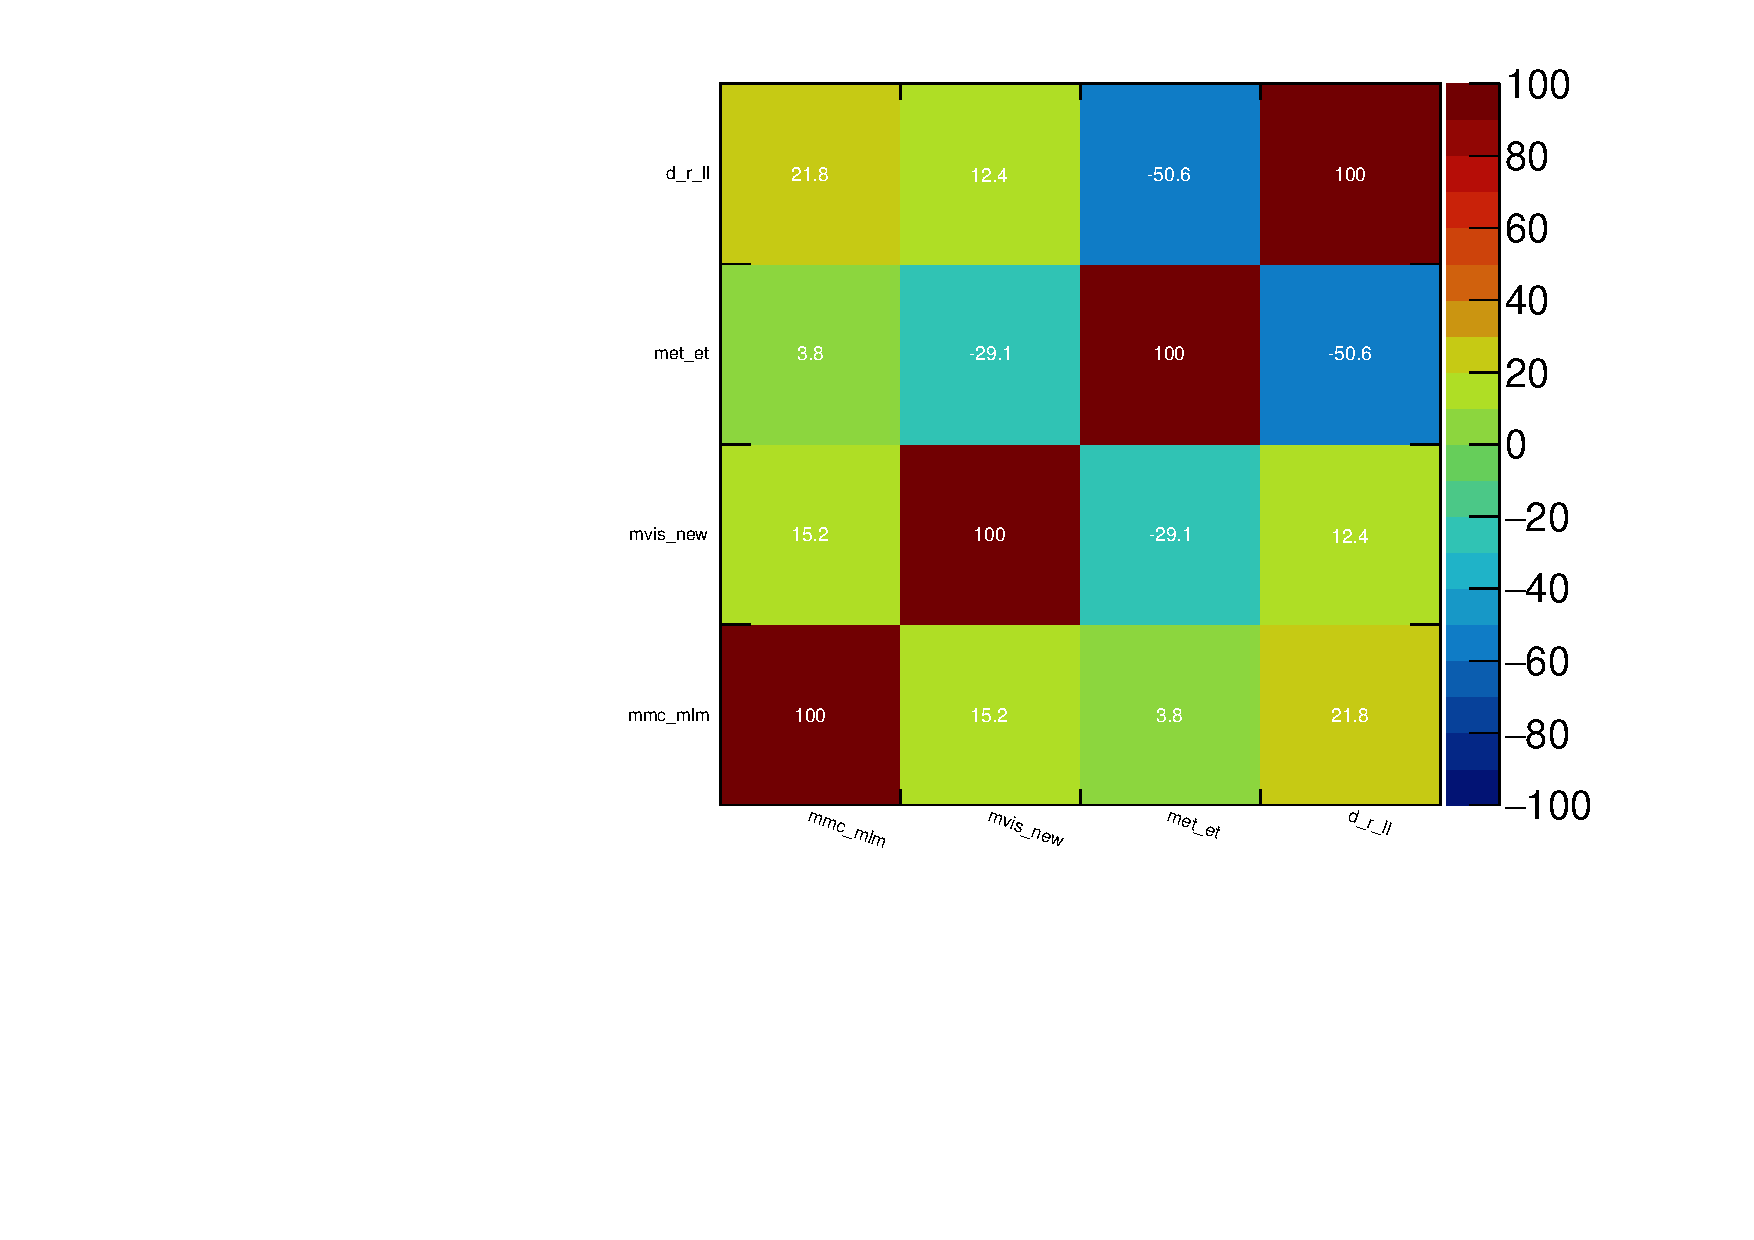
\includegraphics[width=\textwidth]{./plots/mva/variable_reduction/BOOST_SF_CorrelationMatrixS.pdf}
        \caption{Signal.}
    \end{subfigure}
    \begin{subfigure}[t]{0.7\textwidth}
        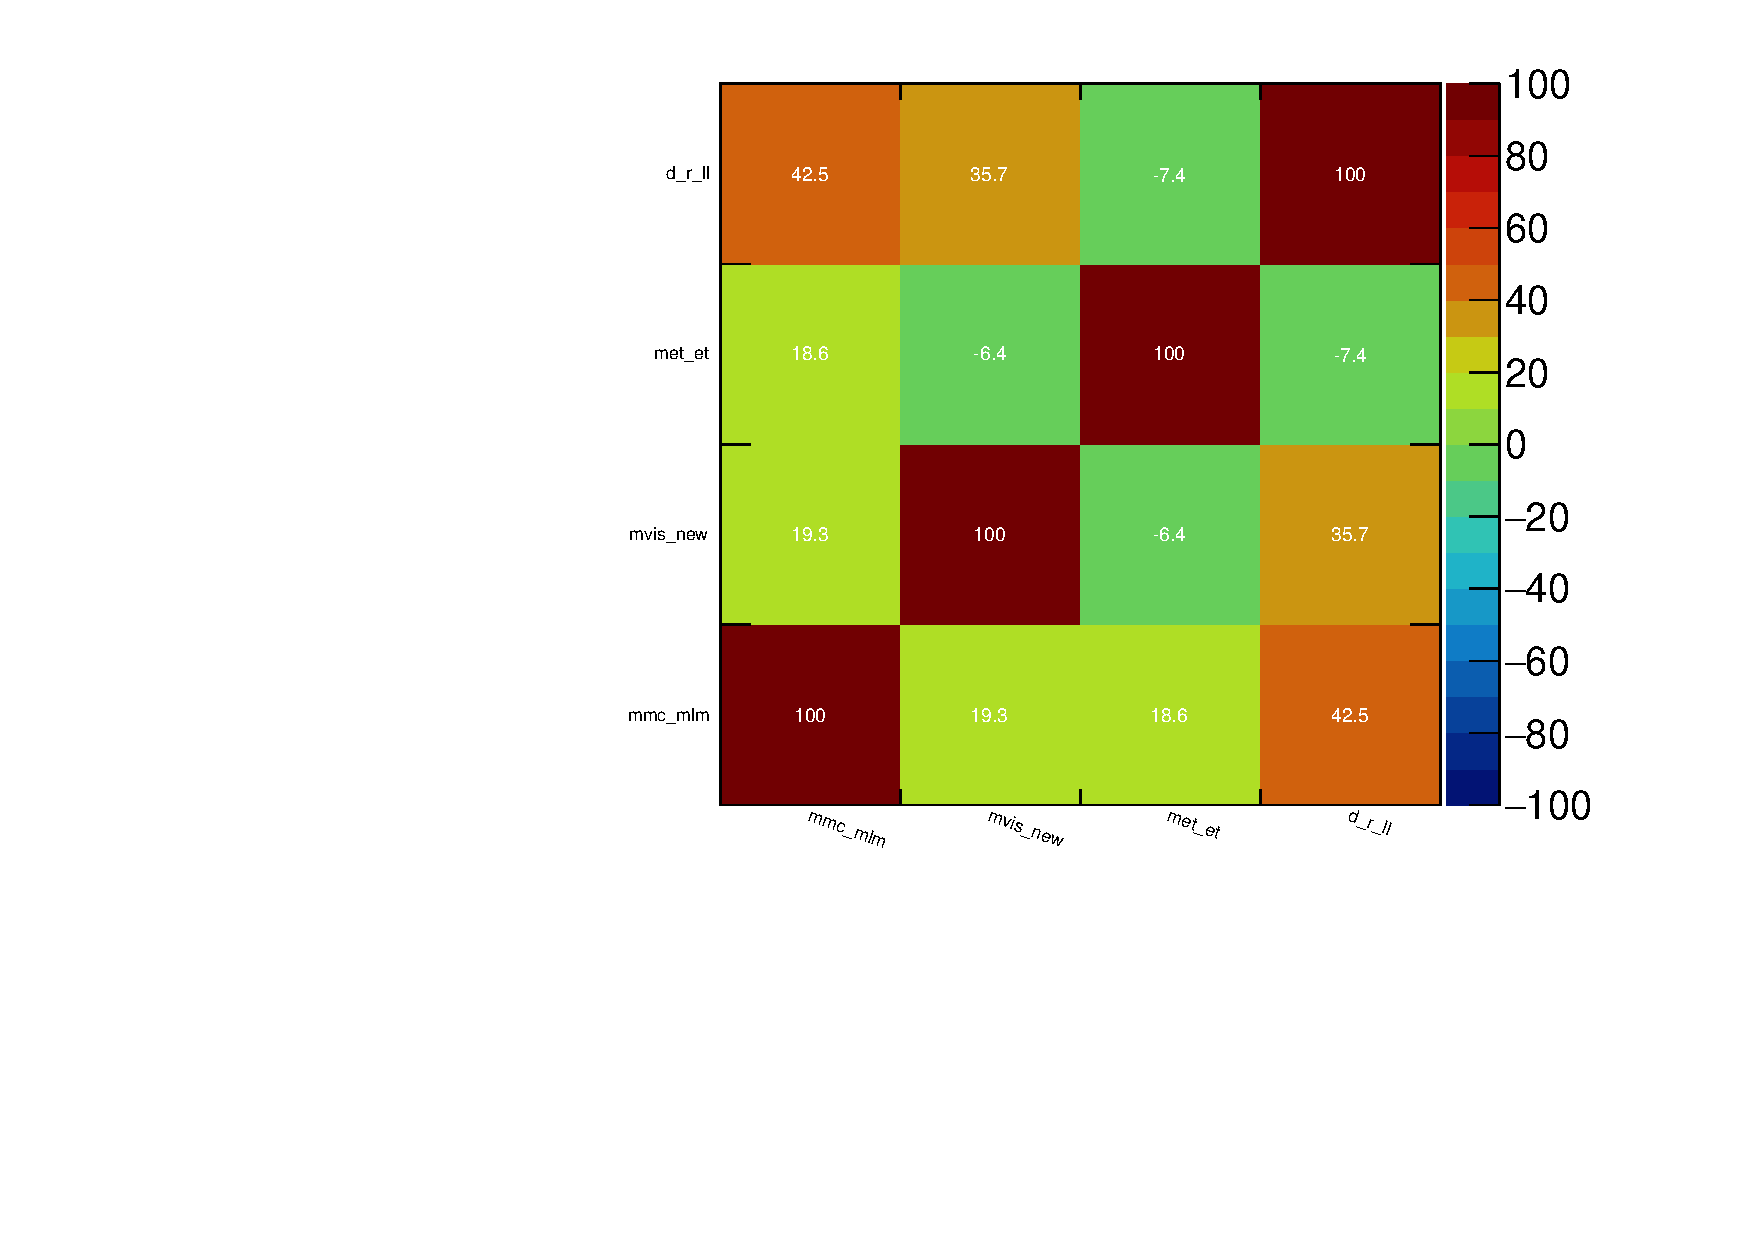
\includegraphics[width=\textwidth]{./plots/mva/variable_reduction/BOOST_SF_CorrelationMatrixB.pdf}
        \caption{Background}
    \end{subfigure}
    \caption{Correlations of the input variables for the BDTs in the boosted SF category for signal and background events.}\label{fig:mva:variables:correlationsb:boostsf}
\end{figure}\begin{figure}[htb]
    \centering
    \begin{subfigure}[t]{0.7\textwidth}
        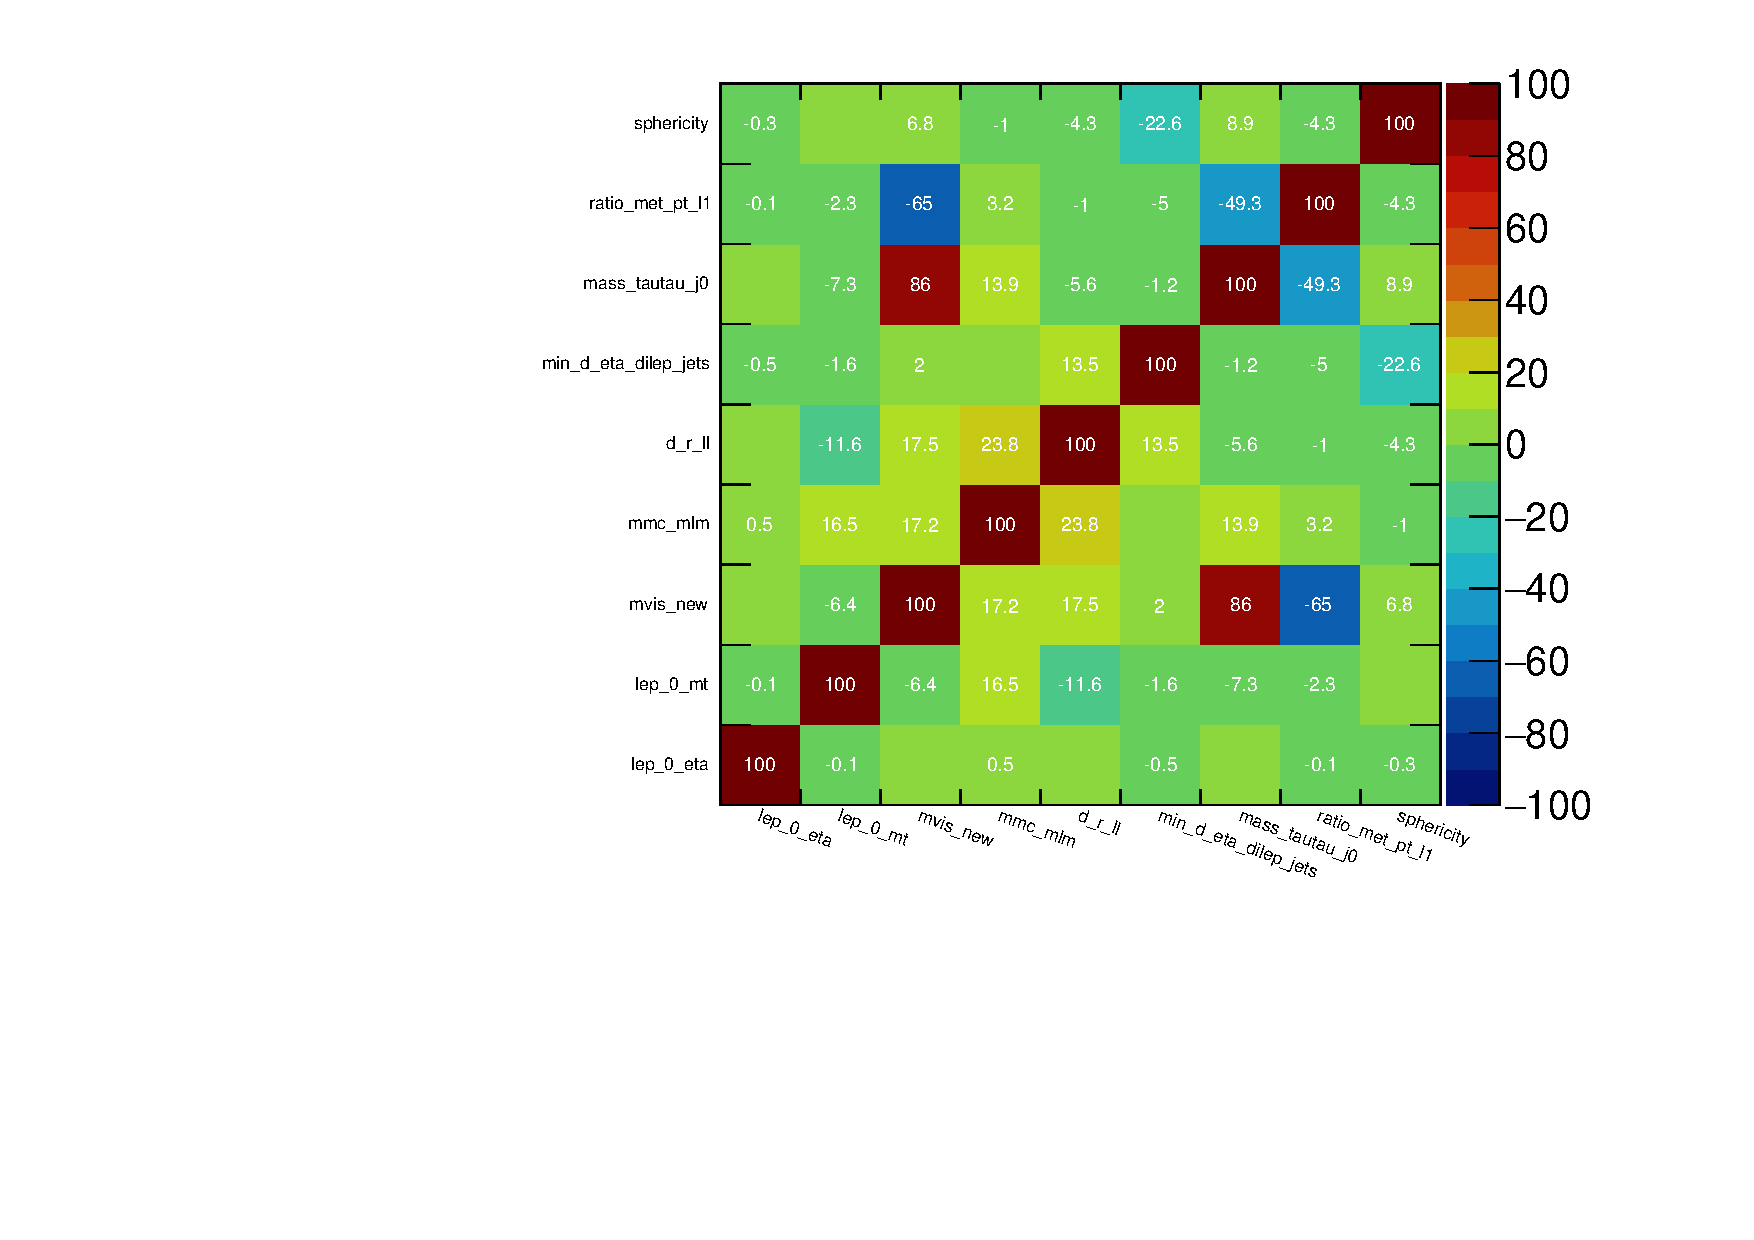
\includegraphics[width=\textwidth]{./plots/mva/variable_reduction/BOOST_DF_CorrelationMatrixS.pdf}
        \caption{Signal.}
    \end{subfigure}
    \begin{subfigure}[t]{0.7\textwidth}
        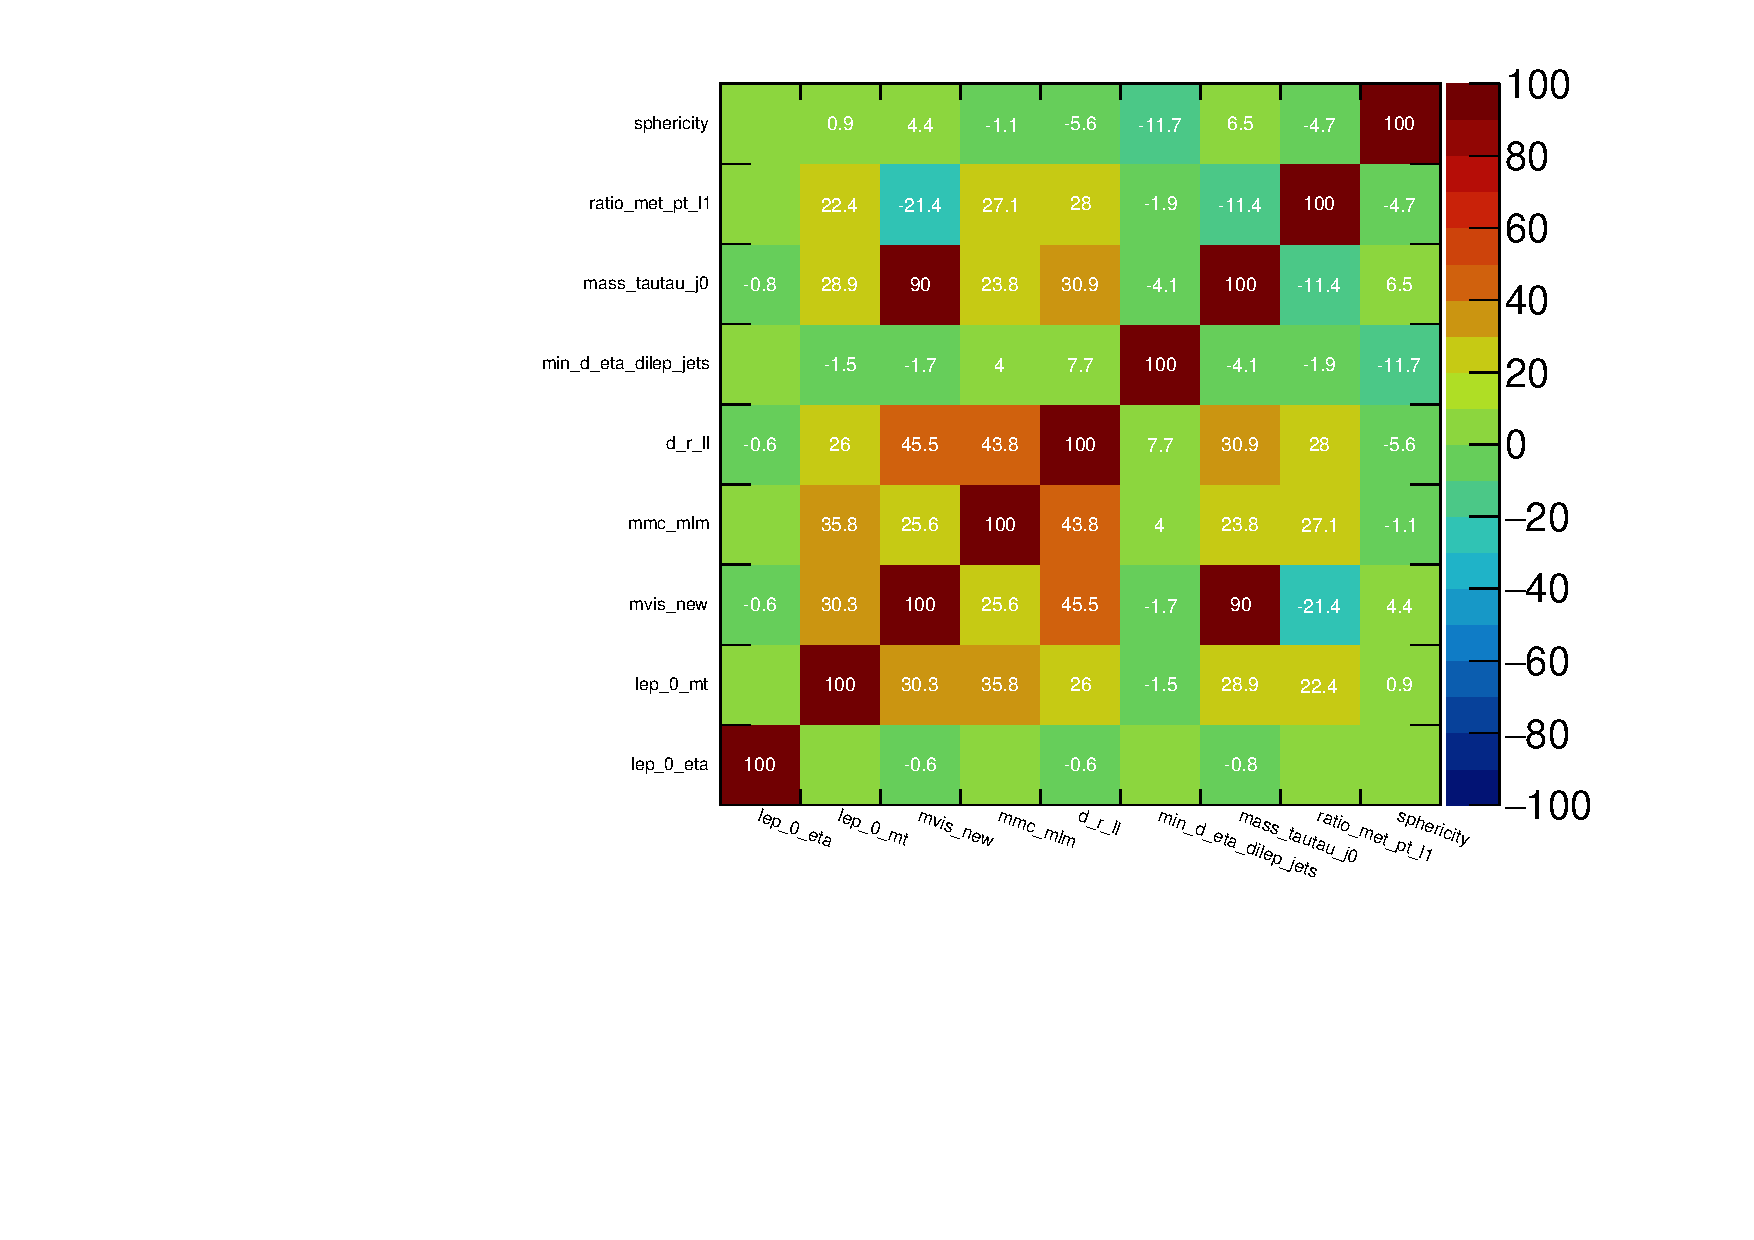
\includegraphics[width=\textwidth]{./plots/mva/variable_reduction/BOOST_DF_CorrelationMatrixB.pdf}
        \caption{Background}
    \end{subfigure}
    \caption{Correlations of the input variables for the BDTs in the boosted DF category for signal and background events.}\label{fig:mva:variables:correlationsb:boostdf}
\end{figure}
